\documentclass[12pt,a4paper]{article}
\usepackage[utf8]{inputenc}
\usepackage[T1]{fontenc}
\usepackage[italian]{babel}
\usepackage{geometry}
\usepackage{amsmath}
\usepackage{amssymb}
\usepackage{listings}
\usepackage{xcolor}
\usepackage{graphicx}
\usepackage{hyperref}
\usepackage{booktabs}
\usepackage{caption}
\usepackage{float}
\usepackage{parskip}
\usepackage{array}
\usepackage{tabularx}
\usepackage{enumitem}
\usepackage{tcolorbox}
\tcbuselibrary{listings,breakable,skins}

\geometry{
  top=2.5cm, bottom=2.5cm,
  left=2.5cm, right=2.5cm
}

\definecolor{codebg}{RGB}{248,248,248}
\definecolor{keywordcolor}{RGB}{0,0,180}
\definecolor{commentcolor}{RGB}{0,128,0}
\definecolor{stringcolor}{RGB}{163,21,21}
\definecolor{codeframe}{RGB}{180,180,180}

\lstdefinestyle{python}{
  language=Python,
  basicstyle=\ttfamily\footnotesize,
  keywordstyle=\color{keywordcolor}\bfseries,
  commentstyle=\color{commentcolor}\itshape,
  stringstyle=\color{stringcolor},
  numberstyle=\tiny\color{gray},
  numbers=left,
  stepnumber=1,
  breaklines=true,
  breakatwhitespace=false,
  showstringspaces=false,
  tabsize=4,
  xleftmargin=1.5em,
  keepspaces=true,
  columns=flexible,
  frame=none,
  aboveskip=0pt,
  belowskip=0pt,
}
\lstset{style=python}

\hypersetup{
  colorlinks=true,
  linkcolor=blue!60!black,
  urlcolor=blue!60!black,
}

\newtcblisting{pylisting}[1][]{
  listing only,
  enhanced,
  colback=codebg,
  colframe=codeframe,
  coltitle=black,
  fonttitle=\small\itshape,
  attach boxed title to top left={yshift=-2mm, xshift=4mm},
  boxed title style={colback=codebg, colframe=codeframe, boxrule=0.5pt},
  boxrule=0.5pt,
  arc=2pt,
  left=4pt, right=4pt, top=8pt, bottom=4pt,
  listing options={style=python},
  before upper={\vspace{-2pt}},
  #1
}

\newtcolorbox{defbox}[1]{colback=blue!5,colframe=blue!60!black,fonttitle=\bfseries,title={#1},breakable}
\newtcolorbox{exbox}[1]{colback=green!5,colframe=green!50!black,fonttitle=\bfseries,title={#1},breakable}
\newtcolorbox{warnbox}[1]{colback=orange!10,colframe=orange!80!black,fonttitle=\bfseries,title={#1},breakable}

\newcommand{\HRule}{\rule{\linewidth}{0.5mm}}

\begin{document}
\raggedbottom

% ============================================================
% FRONTESPIZIO
% ============================================================
\begin{titlepage}
  \centering
  \vspace*{1.2cm}

  {\Large\textbf{Universit\`a degli Studi di Torino}\\[0.3em]
  Corso di Laurea Magistrale in Informatica}

  \vspace{1cm}
  \HRule\\[0.4em]
  {\LARGE\textbf{Tecnologie del Linguaggio Naturale}}\\[0.3em]
  {\large Parte 3 -- Prof.\ Luigi Di Caro}\\[0.2em]
  \HRule

  \vspace{1.2cm}
  {\huge\textbf{Relazione Complessiva}}\\[0.5em]
  {\LARGE Laboratori 1--5}\\[0.6em]
  {\large
    Complessit\`a definizionale e sovrapposizione semantica
    \;$\cdot$\; Ricerca onomasiologica con WordNet
    \;$\cdot$\; Polisemia cross-linguistica
    \;$\cdot$\; Topic modeling con BERTopic
    \;$\cdot$\; Retrieval-Augmented Generation
  }

  \vspace{2cm}

  {\large\textbf{Gruppo di lavoro:}}\\[0.8em]
  \begin{tabular}{ll}
    \toprule
    \textbf{Studente}    & \textbf{Matricola} \\
    \midrule
    Alessandro Olivero   & 915069  \\
    Samuele Iudice       & 1235245 \\
    Andrea Franco        & 1226739 \\
    \bottomrule
  \end{tabular}\\[0.4em]
  {\footnotesize Il Laboratorio 4 \`e stato svolto individualmente da Alessandro Olivero.}

  \vspace{1.5cm}
  \begin{tabular}{ll}
    \textbf{Docente:}          & Prof.\ Luigi Di Caro \\[0.3em]
    \textbf{Anno Accademico:}  & 2025/2026 \\
  \end{tabular}

  \vfill
  {\large \today}
\end{titlepage}

\tableofcontents
\newpage

% ============================================================
\section{Introduzione generale}
% ============================================================

Questa relazione raccoglie e sintetizza i cinque laboratori svolti nella Parte 3 del corso di \textbf{Tecnologie del Linguaggio Naturale} (Prof.\ Luigi Di Caro, A.A.\ 2025/2026). I laboratori, pur affrontando tecniche molto diverse tra loro, seguono un filo conduttore comune: la tensione tra \emph{forma linguistica} e \emph{contenuto semantico}, esplorata a livelli di granularit\`a crescente.

\begin{itemize}
  \item Il \textbf{Lab 1} parte dal problema pi\`u elementare -- definire un concetto in linguaggio naturale -- e misura quanto le definizioni indipendenti di persone diverse si sovrappongano, lessicalmente e semanticamente.
  \item Il \textbf{Lab 2} inverte la prospettiva: data una definizione (il \emph{contenuto}), tenta di risalire automaticamente alla \emph{forma} lessicale corretta codificata in WordNet (ricerca onomasiologica).
  \item Il \textbf{Lab 3} sposta l'analisi sul piano cross-linguistico, mostrando che la complessit\`a polisemica di una parola non \`e una propriet\`a assoluta, ma dipende da come ciascuna lingua organizza il proprio lessico.
  \item Il \textbf{Lab 4} affronta il problema in modo non supervisionato: invece di partire da concetti noti, estrae automaticamente i temi presenti in una grande collezione di documenti (topic modeling) tramite BERTopic.
  \item Il \textbf{Lab 5} chiude il percorso integrando retrieval semantico/lessicale e generazione linguistica in un sistema \textbf{RAG} (Retrieval-Augmented Generation) completo, applicato e valutato su un corpus di paper scientifici NLP.
\end{itemize}

Tutti i laboratori condividono inoltre un dataset o una risorsa lessicale di riferimento (il dataset di definizioni raccolto in aula per i Lab 1--2, WordNet/OMW per i Lab 1--3, il corpus \texttt{arXiv-NLP} per i Lab 4--5), il che permette confronti diretti tra i risultati, evidenziati nelle sezioni di discussione di ciascun laboratorio.

% ============================================================
\section{Lab 1 -- Complessit\`a Definizionale e Sovrapposizione Semantica}
% ============================================================

\subsection{Obiettivo e materiale}

L'obiettivo del Lab 1 \`e esplorare la complessit\`a insita nella formulazione di definizioni in linguaggio naturale, per quattro concetti bilanciati lungo due dimensioni (concretezza e specificit\`a):

\begin{itemize}[noitemsep]
  \item \textbf{Tree} (Albero): concreto, generico.
  \item \textbf{Teapot} (Teiera): concreto, specifico.
  \item \textbf{Music} (Musica): astratto, generico.
  \item \textbf{Ethics} (Etica): astratto, specifico.
\end{itemize}

\`E stato utilizzato un dataset (\texttt{Dataset definizioni-spurio.csv}) contenente le definizioni in linguaggio naturale raccolte in aula da studenti diversi per ciascuno dei quattro concetti, con il vincolo che ogni definizione fosse comprensibile a un lettore generico.

\subsection{Analisi qualitativa}

Dall'analisi delle definizioni raccolte emergono tre dinamiche linguistiche rilevanti:

\begin{enumerate}[noitemsep]
  \item \textbf{Scelte lessicali e specificit\`a}: per i concetti concreti il lessico si concentra su componenti fisiche e funzionali (\textit{roots}, \textit{metal container}); per i concetti astratti il vocabolario si sposta sulla sfera cognitiva e sensoriale (\textit{sentiment}, \textit{behavior}, \textit{melodious sounds}).
  \item \textbf{Difficolt\`a concettuale}: i concetti astratti generano definizioni pi\`u eterogenee e dipendenti dal contesto socio-culturale, mentre per i concetti concreti il referente fisico guida in modo pi\`u uniforme la descrizione.
  \item \textbf{Strategie definitorie}: lo schema aristotelico \emph{genus-differentia} \`e adottato spontaneamente per i concetti concreti (\textit{Tree} = \textit{kind of plant} [genus] + \textit{composed by a trunk} [differentia]), mentre per i concetti astratti prevalgono parafrasi operative basate sull'effetto prodotto.
\end{enumerate}

\subsection{Metodologia quantitativa}

Per quantificare la sovrapposizione tra le definizioni di uno stesso concetto sono state applicate due metriche, calcolate a coppie su tutte le definizioni disponibili per ciascun concetto:

\begin{itemize}
  \item \textbf{Simlex (Jaccard)}: il testo viene normalizzato (minuscolo, rimozione di punteggiatura e stopword, lemmatizzazione) e si calcola l'indice di Jaccard tra gli insiemi di parole di ogni coppia di definizioni.
  \item \textbf{Simsem (Cosine su TF-IDF)}: le definizioni vengono vettorizzate con TF-IDF e si calcola la cosine similarity media tra tutte le coppie, per catturare la vicinanza concettuale anche in assenza di sovrapposizione lessicale esatta.
\end{itemize}

\begin{pylisting}[title={Indice di Jaccard tra definizioni normalizzate}]
def jaccard_similarity(set1, set2):
    if not set1 or not set2:
        return 0.0
    intersection = len(set1.intersection(set2))
    union = len(set1.union(set2))
    return intersection / union
\end{pylisting}

\subsection{Risultati}

\begin{table}[H]
  \centering
  \caption{Sovrapposizione lessicale (Simlex) e semantica (Simsem) media, per concetto}
  \begin{tabular}{lllcc}
    \toprule
    \textbf{Concetto} & \textbf{Tipo} & \textbf{Specificit\`a} & \textbf{Simlex (Jaccard)} & \textbf{Simsem (Cosine)} \\
    \midrule
    Tree   & Concreto & Generico  & 0.084 & 0.077 \\
    Teapot & Concreto & Specifico & 0.057 & 0.062 \\
    Ethics & Astratto & Specifico & 0.034 & 0.041 \\
    Music  & Astratto & Generico  & 0.034 & 0.036 \\
    \bottomrule
  \end{tabular}
\end{table}

\subsection{Discussione}

\begin{itemize}
  \item \textbf{Variabilit\`a lessicale altissima}: i valori di Jaccard sono estremamente bassi per tutti i concetti (massimo 8.4\% per \textit{Tree}), a dimostrazione che parlanti diversi scelgono vocaboli molto diversi anche descrivendo lo stesso referente.
  \item \textbf{Il coseno TF-IDF compensa parzialmente la variabilit\`a lessicale}: per i concetti astratti (\textit{Ethics}, \textit{Music}) la similarit\`a semantica supera quella lessicale, perch\'e il TF-IDF allinea parzialmente sinonimi e termini affini che il solo confronto insiemistico non cattura.
  \item \textbf{Concretezza vs astrazione}: emerge un pattern netto -- i concetti concreti ottengono punteggi di similarit\`a sistematicamente superiori. Il referente fisico vincola il lessico condiviso dai parlanti, mentre l'astrazione concettuale amplifica le divergenze interpretative.
\end{itemize}

Questo ultimo punto -- il ruolo stabilizzante del referente fisico concreto -- ricorrer\`a anche nel Lab 2 (accuratezza di recupero pi\`u alta per concetti concreti) e nel Lab 3 (minore asimmetria cross-linguistica per sostantivi concreti come \textit{mouth} e \textit{table}).

% ============================================================
\section{Lab 2 -- Valutazione Content-to-Form: Ricerca Onomasiologica con WordNet}
% ============================================================

\subsection{Obiettivo}

Il Lab 2 esplora la \textbf{ricerca onomasiologica}: dato un contenuto (una definizione in linguaggio naturale, le stesse raccolte nel Lab 1), si cerca di risalire alla forma lessicale codificata in WordNet, ovvero al synset corretto. Si inverte cos\`i la direzione tipica di un dizionario (forma $\to$ contenuto), chiedendosi: \emph{quanto deve essere ``buona'' una definizione perch\'e permetta il recupero automatico del concetto giusto?}

\subsection{Metodo}

Per ciascuno dei quattro concetti (\textit{Music}, \textit{Ethics}, \textit{Tree}, \textit{Teapot}) sono stati selezionati da WordNet 3.1 i 5 synset candidati pi\`u plausibili (incluso il synset target corretto, sensi alternativi e iperonimi). Per ciascuna delle 28 definizioni del dataset si applica la procedura:

\begin{enumerate}[noitemsep]
  \item Pulizia del testo: minuscolo, rimozione di punteggiatura e stopword.
  \item Vettorizzazione TF-IDF della definizione e delle 5 glosse candidate.
  \item Selezione del synset con cosine similarity pi\`u alta rispetto alla definizione.
  \item Confronto con il synset target per determinare se il recupero \`e corretto.
\end{enumerate}

\begin{pylisting}[title={Selezione del synset per cosine similarity TF-IDF}]
corpus = [defn_clean] + glosses_clean
tfidf  = TfidfVectorizer()
mat    = tfidf.fit_transform(corpus)
sims   = cosine_similarity(mat[0:1], mat[1:])[0]
best_synset = syn_names[int(np.argmax(sims))]
correct     = (best_synset == target_syn)
\end{pylisting}

\subsection{Risultati}

\begin{table}[H]
  \centering
  \caption{Accuratezza e score di similarit\`a per concetto (28 definizioni totali)}
  \begin{tabular}{llp{2.3cm}lrr}
    \toprule
    \textbf{Concetto} & \textbf{Tipo} & \textbf{Specificit\`a} & \textbf{Sintet target} & \textbf{Corretto} & \textbf{Score medio} \\
    \midrule
    Music  & Astratto & Generico  & \texttt{music.n.01}  & 9/28 (32.1\%)  & 0.130 \\
    Ethics & Astratto & Specifico & \texttt{ethics.n.01} & 12/28 (42.9\%) & 0.152 \\
    Tree   & Concreto & Generico  & \texttt{tree.n.01}   & 25/28 (89.3\%) & 0.103 \\
    Teapot & Concreto & Specifico & \texttt{teapot.n.01} & 20/28 (71.4\%) & 0.127 \\
    \bottomrule
  \end{tabular}
\end{table}

\begin{table}[H]
  \centering
  \caption{Aggregazione per tipo e specificit\`a}
  \begin{tabular}{llrr}
    \toprule
    \textbf{Dimensione} & \textbf{Gruppo} & \textbf{Score medio} & \textbf{Accuratezza} \\
    \midrule
    Tipo          & Astratto  & 0.141 & 37.5\% \\
    Tipo          & Concreto  & 0.115 & 80.4\% \\
    Specificit\`a & Generico  & 0.116 & 60.7\% \\
    Specificit\`a & Specifico & 0.140 & 57.1\% \\
    \bottomrule
  \end{tabular}
\end{table}

\subsection{Discussione}

\paragraph{Concreto vs astratto.} Il risultato pi\`u significativo \`e la netta differenza di accuratezza tra concetti concreti (80.4\%) e astratti (37.5\%). I concetti concreti hanno propriet\`a fisiche ben definite che si traducono in un vocabolario condiviso e prevedibile tra gli studenti, facilitando il matching con le glosse WordNet; i concetti astratti ammettono invece angolature molto diverse (emotiva, filosofica, strutturale), per cui il TF-IDF non riesce a catturare la somiglianza concettuale quando le parole usate divergono.

\paragraph{L'efficacia dello schema genus-differentia.} Le definizioni che seguono esplicitamente lo schema \emph{genus-differentia} ottengono sistematicamente score pi\`u alti: ad esempio la definizione di \textit{Ethics} con score 0.63 (\textit{``branch of philosophy [genus] that studies human behavior by trying to define what is right and what is wrong [differentia]''}) si allinea quasi letteralmente con la glossa di \texttt{ethics.n.01}.

\paragraph{Limiti del TF-IDF.} Il metodo presenta tre limiti rilevanti: \emph{opacit\`a semantica} (sinonimi come \textit{container} e \textit{vessel} non vengono riconosciuti come simili), \emph{sensibilit\`a alla lunghezza} (definizioni brevi producono vettori sparsi) e \emph{assenza di struttura sintattica} (bag-of-words, mentre lo schema genus-differentia ha una struttura semanticamente significativa). Un approccio con embedding contestuali (es.\ Sentence-BERT) supererebbe il limite della dipendenza lessicale esatta -- esattamente l'approccio poi adottato nei Lab 4 e 5.

% ============================================================
\section{Lab 3 -- Complessit\`a Polisemica Cross-Linguistica}
% ============================================================

\subsection{Obiettivo}

Il Lab 3 verifica empiricamente la tesi secondo cui \textbf{la polisemia non \`e una propriet\`a universale della parola, ma del modo in cui una lingua organizza il proprio lessico}: la stessa area concettuale pu\`o essere lessicalizzata in modo completamente diverso da una lingua all'altra. Si confronta la complessit\`a polisemica di \textbf{20 lemmi} (8 sostantivi, 6 verbi, 6 aggettivi) tradotti in \textbf{inglese, italiano e spagnolo}, usando l'Open Multilingual WordNet (OMW) tramite NLTK.

\subsection{Metodologia}

Per ogni lemma e lingua si recuperano i synset con \texttt{wn.synsets(lemma, lang=...)} e si conta il numero di sensi $N(w)$. Poich\'e OMW non fornisce frequenze d'uso per le lingue non inglesi (a differenza dell'inglese, dove esistono dati SemCor), si assume una \textbf{distribuzione uniforme} sui sensi disponibili, per cui l'entropia di Shannon si riduce a $H(w) = \log_2 N(w)$: una scala pi\`u interpretabile del conteggio grezzo, ma non una misura indipendente da esso -- un limite esplicito del dataset multilingue, discusso criticamente nella relazione originale.

L'\textbf{asimmetria} cross-linguistica di un lemma \`e definita come
\[
  \text{asimmetria}(w) = \max(N_{en}, N_{it}, N_{es}) - \min(N_{en}, N_{it}, N_{es}).
\]

\subsection{Risultati}

\begin{table}[H]
  \centering
  \caption{Statistiche aggregate sui 20 lemmi, per lingua}
  \begin{tabular}{lrrrrr}
    \toprule
    \textbf{Lingua} & \textbf{Media sensi} & \textbf{Mediana} & \textbf{Max} & \textbf{Media entropia} \\
    \midrule
    Inglese  & 31.70 & 30.5 & 75 & 4.79 bit \\
    Italiano &  7.95 &  6.5 & 23 & 2.71 bit \\
    Spagnolo & 13.15 & 12.5 & 32 & 3.45 bit \\
    \bottomrule
  \end{tabular}
\end{table}

\begin{figure}[H]
  \centering
  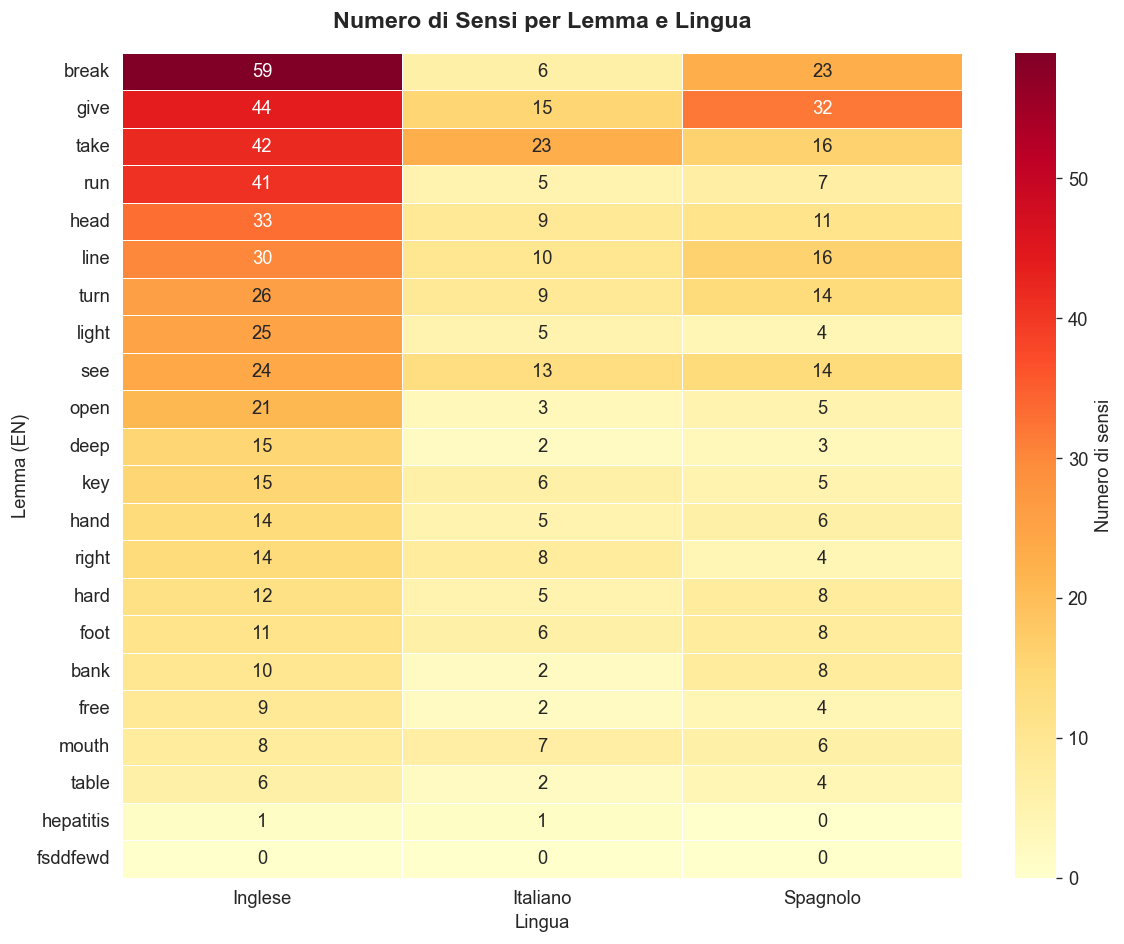
\includegraphics[width=0.85\textwidth]{heatmap_sensi.png}
  \caption{Numero di sensi per ciascuno dei 20 lemmi nelle tre lingue (ordinati per numero di sensi in inglese, decrescente).}
\end{figure}

\begin{table}[H]
  \centering
  \caption{Top 5 lemmi per asimmetria cross-linguistica (max$-$min sensi)}
  \begin{tabular}{lrrrr}
    \toprule
    \textbf{Lemma (EN)} & \textbf{Inglese} & \textbf{Italiano} & \textbf{Spagnolo} & \textbf{Asimmetria} \\
    \midrule
    break & 75 & 6  & 23 & 69 \\
    run   & 57 & 5  & 7  & 52 \\
    light & 47 & 5  & 17 & 42 \\
    head  & 42 & 9  & 11 & 33 \\
    open  & 36 & 4  & 24 & 32 \\
    \bottomrule
  \end{tabular}
\end{table}

\begin{figure}[H]
  \centering
  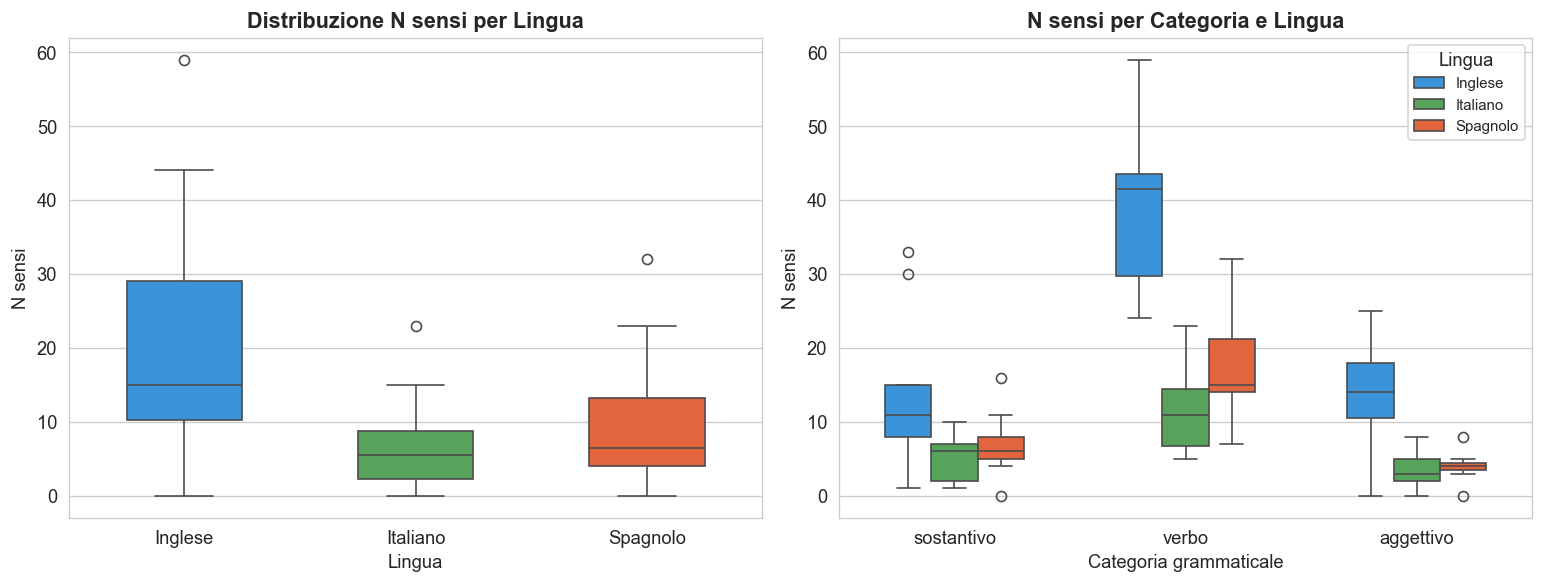
\includegraphics[width=0.95\textwidth]{boxplot_distribuzione.png}
  \caption{Sinistra: distribuzione del numero di sensi per lingua. Destra: distribuzione per categoria grammaticale.}
\end{figure}

\subsection{Discussione}

\paragraph{Gerarchia EN $\gg$ ES $>$ IT.} In media l'inglese registra circa 4 volte pi\`u sensi dell'italiano e oltre il doppio dello spagnolo, per lo stesso lemma. Il pattern si mantiene all'interno di ogni categoria grammaticale, ma va interpretato con cautela: Princeton WordNet \`e una risorsa raffinata da oltre 30 anni con granularit\`a dei sensi molto fine, mentre le estensioni OMW per italiano e spagnolo sono mappature pi\`u recenti e meno esaustive. Parte della differenza \`e quindi attribuibile a copertura/granularit\`a delle risorse, non solo a una reale differenza di polisemia.

\paragraph{Il caso \textit{bank}: asimmetria strutturale, non solo quantitativa.} In italiano ``banca'' (2 sensi) copre quasi solo l'istituto finanziario (il senso ``riva del fiume'' \`e lessicalizzato come \textit{riva}); in spagnolo ``banco'' (8 sensi) \`e pi\`u carico semanticamente, includendo anche il mobile e il banco di sabbia/pesci -- pi\`u vicino al comportamento inglese. La stessa area concettuale viene quindi ripartita diversamente tra le tre lingue.

\paragraph{Verbi vs sostantivi concreti.} I lemmi con asimmetria massima sono entrambi verbi (\textit{run}, \textit{break}), che in inglese si estendono a domini semantici eterogenei lessicalizzati in italiano/spagnolo con verbi distinti. All'opposto, sostantivi concreti con referente fisico stabile (\textit{mouth}, \textit{table}) mostrano la minore asimmetria -- lo stesso effetto stabilizzante del referente concreto osservato nei Lab 1--2.

\paragraph{Implicazioni per l'NLP multilingue.} Un sistema di machine translation o cross-lingual transfer che assuma una corrispondenza 1:1 tra i sensi di un lemma inglese e del suo corrispettivo italiano/spagnolo commetterebbe un errore sistematico, specialmente per verbi ad alta polisemia.

Il limite principale \`e l'assunzione di distribuzione uniforme dei sensi, dovuta all'assenza di dati di frequenza d'uso in OMW per le lingue romanze.

% ============================================================
\section{Lab 4 -- Topic Modeling con BERTopic}
% ============================================================

\textit{Laboratorio svolto individualmente da Alessandro Olivero.}

\subsection{Obiettivo}

Costruire una pipeline completa di \textbf{topic modeling non supervisionato} sul dataset \texttt{MaartenGr/arxiv\_nlp} (44.949 abstract di paper NLP da arXiv, senza etichette tematiche), confrontando almeno tre configurazioni che variano modello di embedding, parametri UMAP e parametri HDBSCAN.

\subsection{Architettura della pipeline}

\begin{enumerate}[noitemsep]
  \item \textbf{Embedding}: ogni abstract \`e convertito in un vettore denso con un modello SentenceTransformer.
  \item \textbf{UMAP}: riduzione dimensionale che preserva la struttura semantica locale/globale.
  \item \textbf{HDBSCAN}: clustering density-based, etichetta $-1$ per gli outlier.
  \item \textbf{BERTopic}: estrae parole rappresentative per ciascun cluster tramite c-TF-IDF (TF-IDF contestualizzato per cluster).
\end{enumerate}

\subsection{Configurazioni testate}

\begin{table}[H]
  \centering
  \small
  \caption{Le tre configurazioni confrontate}
  \begin{tabular}{p{2.6cm}p{3.1cm}p{4.3cm}p{3.6cm}}
    \toprule
    \textbf{Config} & \textbf{Embedding} & \textbf{UMAP} & \textbf{HDBSCAN} \\
    \midrule
    1 -- Baseline       & \texttt{gte-small} (384d)     & n\_comp=5, n\_neigh=15   & min\_cluster=50 \\
    2 -- MiniLM fine    & \texttt{all-MiniLM-} \texttt{L6-v2}     & n\_comp=10, n\_neigh=10  & min\_cluster=30 \\
    3 -- MiniLM coarse  & \texttt{all-MiniLM-} \texttt{L6-v2}     & n\_comp=5, n\_neigh=30   & min\_cluster=150 \\
    \bottomrule
  \end{tabular}
\end{table}

\subsection{Risultati}

\begin{table}[H]
  \centering
  \caption{Confronto quantitativo tra le tre configurazioni}
  \begin{tabular}{lrrrl}
    \toprule
    \textbf{Configurazione} & \textbf{\#Topic} & \textbf{Outlier} & \textbf{Outlier\%} & \textbf{Tempo totale} \\
    \midrule
    1 -- Baseline      & 151 & 14.357 & 31.9\% & $\approx$ 3h 47m \\
    2 -- MiniLM fine   & 171 & 12.747 & 28.4\% & $\approx$ 17m 30s \\
    3 -- MiniLM coarse &  49 & 14.899 & 33.1\% & $\approx$ 11m \\
    \bottomrule
  \end{tabular}
\end{table}

\begin{exbox}{Esempio -- Config 1 (Baseline), top-5 topic per numero documenti}
\begin{verbatim}
0  2235  speech, asr, recognition, end, acoustic
1  2166  question, qa, questions, answer, answering
2  1603  medical, clinical, biomedical, patient, health
3   886  summarization, summaries, summary, abstractive
4   862  translation, nmt, machine, bleu, neural
\end{verbatim}
\end{exbox}

\subsection{Discussione}

\paragraph{Config 1 vs Config 2: granularit\`a e qualit\`a.} Entrambe producono topic semanticamente coerenti e privi di stopword. La Config 2 produce 20 topic in pi\`u (171 vs 151) e meno outlier (28.4\% vs 31.9\%): \texttt{min\_cluster\_size=30} pi\`u basso consente cluster pi\`u piccoli e numerosi, mentre \texttt{n\_components=10} preserva pi\`u struttura semantica locale. Computazionalmente la differenza \`e enorme: la Config 1 richiede $\approx$3h47m (13.484s solo per gli embedding con \texttt{gte-small} su CPU), la Config 2 meno di 18 minuti -- a parit\`a (o superiorit\`a) di qualit\`a, \texttt{all-MiniLM-L6-v2} \`e la scelta pi\`u efficiente per dataset di questa dimensione senza GPU.

\paragraph{Config 3: un failure mode istruttivo.} Con \texttt{min\_cluster\_size=150} e \texttt{n\_neighbors=30}, HDBSCAN forma solo 49 cluster molto pi\`u grandi e tematicamente misti. Il c-TF-IDF, calcolato su cluster troppo eterogenei, diluisce le parole discriminanti con termini ad alta frequenza globale -- incluse le stopword: i topic risultanti contengono esplicitamente \textit{the}, \textit{to}, \textit{and}, \textit{of} tra le prime cinque parole (es.\ topic ``transformer, attention, \textbf{the}, models, \textbf{of}''), segno che il segnale semantico specifico del cluster \`e insufficiente rispetto al rumore introdotto dalla dimensione eccessiva.

\paragraph{Configurazione consigliata.} La Config 2 risulta complessivamente la migliore: pi\`u topic, meno outlier, parole rappresentative pulite, tempo di esecuzione praticabile su CPU. Il laboratorio mostra come la qualit\`a del topic modeling dipenda criticamente dalla combinazione di tre fattori -- capacit\`a dell'embedding di catturare la semantica del dominio, granularit\`a della proiezione UMAP, soglia di densit\`a di HDBSCAN -- e come anche tecniche moderne come BERTopic non siano esenti da failure mode prevedibili e analizzabili.

% ============================================================
\section{Lab 5 -- Retrieval-Augmented Generation (RAG)}
% ============================================================

\subsection{Obiettivo}

Il Lab 5 integra retrieval e generazione in un sistema \textbf{RAG} completo sul medesimo corpus arXiv-NLP, confrontando due strategie di retrieval:

\begin{itemize}[noitemsep]
  \item \textbf{RAG base}: retrieval puramente semantico (SciBERT + FAISS).
  \item \textbf{RAG ibrido}: fusione di retrieval semantico e lessicale (BM25), tramite Reciprocal Rank Fusion (RRF).
\end{itemize}

Entrambe le pipeline generano la risposta finale con \textbf{Phi-3.5-mini-instruct} (Microsoft, 3.8B parametri), condizionato sui documenti recuperati.

\subsection{Architettura}

\begin{enumerate}[noitemsep]
  \item \textbf{Retrieval semantico}: SciBERT (\texttt{allenai/scibert\_scivocab\_uncased}, pre-addestrato su 1.14M paper scientifici) codifica query e documenti in vettori a 768 dimensioni, normalizzati per similarit\`a coseno; FAISS \texttt{IndexFlatIP} esegue la ricerca esatta.
  \item \textbf{Retrieval lessicale (solo ibrido)}: BM25Okapi, efficace sui termini tecnici esatti (es.\ ``NER'', ``LDA'') che SciBERT tende a generalizzare.
  \item \textbf{Fusione RRF (solo ibrido)}: $\text{RRF}(d) = \sum_r \frac{1}{k + \text{rank}_r(d)}$ con $k=60$, applicata ai top-20 di ciascun retriever.
  \item \textbf{Generazione}: Phi-3.5-mini-instruct riceve query + documenti come contesto (troncato a 3000 caratteri) e genera la risposta citando le fonti (\texttt{[Paper X]}), con temperatura $T=0.3$.
\end{enumerate}

\begin{pylisting}[title={Retrieval ibrido con Reciprocal Rank Fusion}]
def retrieve_hybrid(query, faiss_index, bm25, documents, metadata, k=5):
    sem = retrieve_semantic(query, faiss_index, documents, metadata, k=20)
    bm  = retrieve_bm25(query, bm25, documents, metadata, k=20)
    return reciprocal_rank_fusion([sem, bm])[:k]
\end{pylisting}

\subsection{Metriche di valutazione (ispirate a RAGAS)}

\begin{itemize}[noitemsep]
  \item \textbf{Precision@k}: quota di documenti rilevanti (per gold standard a parole chiave) tra i top-$k$ recuperati.
  \item \textbf{Context Relevance}: coseno medio tra l'embedding della query e gli snippet dei documenti recuperati.
  \item \textbf{Answer Relevance}: coseno tra l'embedding della query e quello della risposta generata.
  \item \textbf{Faithfulness proxy}: quota di parole contenutistiche della risposta presenti nel testo dei documenti di contesto.
  \item \textbf{Robustezza}: overlap@5 tra i risultati di una query e quelli delle sue parafrasature.
\end{itemize}

\subsection{Esperimento 1: variazione della dimensione del corpus (RAG base vs ibrido)}

Il corpus \`e stato fatto variare su cinque dimensioni $N_{\text{DOCS}} \in \{1\,000, 5\,000, 15\,000, 25\,000, 44\,949\}$ (corpus completo), ricostruendo gli indici e ripetendo la valutazione su 5 query gold standard.

\begin{table}[H]
  \centering
  \caption{Precision@5 al variare di N\_DOCS: RAG base vs ibrido}
  \begin{tabular}{rrrrr}
    \toprule
    \textbf{N\_DOCS} & \textbf{Base} & \textbf{Ibrido} & \textbf{Delta} & \textbf{Miglioramento} \\
    \midrule
    1\,000  & 0.160 & 0.400 & +0.240 & +150.0\% \\
    5\,000  & 0.240 & 0.560 & +0.320 & +133.3\% \\
    15\,000 & 0.160 & 0.520 & +0.360 & +225.0\% \\
    25\,000 & 0.200 & 0.440 & +0.240 & +120.0\% \\
    44\,949 & 0.120 & 0.360 & +0.240 & +200.0\% \\
    \bottomrule
  \end{tabular}
\end{table}

Il retrieval ibrido supera il baseline semantico in \emph{tutte e cinque} le configurazioni (+120\% a +225\%): BM25 recupera i paper con terminologia tecnica esatta che SciBERT generalizza eccessivamente, e RRF bilancia i due segnali. La Precision@5 ibrida non cresce monotonamente con $N_{\text{DOCS}}$: picco a 5\,000 documenti (0.560), calo a 44\,949 (0.360) -- corpus molto grandi aumentano il ``rumore'' nel retrieval per entrambi i retriever. La Faithfulness proxy \`e sistematicamente pi\`u alta per il sistema ibrido ($+0.027$ a $+0.095$), segno di risposte pi\`u ancorate al contesto tecnico recuperato. La Robustezza (overlap@5 su query parafrasate) \`e invece inversamente correlata a $N_{\text{DOCS}}$ (da 0.233 a $N=1\,000$ a $\sim$0 per corpus grandi): con pi\`u documenti, piccole variazioni lessicali della query spostano sensibilmente i confini di un denso spazio di candidati.

\subsection{Esperimento 2: variazione del parametro k e qualit\`a su query eterogenee}

Una domanda diretta del Prof.\ Di Caro durante la revisione del progetto chiedeva se fossero stati provati valori di $k$ diversi da 5, e se il sistema fosse stato testato con domande diverse valutandone la qualit\`a. Lo script del RAG base \`e stato quindi esteso con un confronto su $k \in \{3, 5, 10, 15\}$ su un insieme di \textbf{7 query eterogenee} (oltre a BERT/attention e word2vec, anche topic modeling, NER, sentiment analysis, dependency parsing, machine translation), a $N_{\text{DOCS}}=15\,000$:

\begin{table}[H]
  \centering
  \caption{Precision@k e Context Relevance al variare di k (RAG base, 7 query, N\_DOCS=15\,000)}
  \begin{tabular}{rrr}
    \toprule
    \textbf{k} & \textbf{Precision@k} & \textbf{Context Relevance} \\
    \midrule
    3  & 0.238 & 0.719 \\
    5  & 0.314 & 0.719 \\
    10 & 0.314 & 0.719 \\
    15 & 0.295 & 0.719 \\
    \bottomrule
  \end{tabular}
\end{table}

$k=5$ risulta il miglior compromesso (in pareggio con $k=10$): aumentare $k$ oltre 5--10 non migliora la precisione media e la peggiora leggermente a $k=15$, perch\'e i documenti aggiuntivi sono in media meno rilevanti. La Context Relevance resta costante perch\'e \`e calcolata sugli stessi vettori SciBERT usati per il ranking: i primi $k$ risultati restano, in aggregato, ugualmente vicini alla query indipendentemente da quanti ne vengano restituiti.

\begin{warnbox}{Un limite osservato concretamente: la query su BERT}
Per la query \textit{``What is BERT and how does self-attention work?''}, il retrieval semantico puro (a $N_{\text{DOCS}}=15\,000$) recupera paper completamente fuori tema (es.\ su dialogue scorekeeping o cognitive issues in NLP), mancando i paper specifici su BERT. L'LLM, correttamente, riconosce l'assenza di informazione pertinente nel contesto e lo dichiara esplicitamente invece di generare contenuto allucinato -- un comportamento di \emph{faithfulness} corretto, ma che evidenzia lo stesso limite del retrieval semantico puro gi\`a osservato nell'Esperimento 1: \`e esattamente la ragione per cui la versione ibrida (Sez.~7.4) aggiunge BM25.
\end{warnbox}

Lo script \`e stato inoltre strutturato per ripetere questo confronto su k a tutte le dimensioni di corpus dell'Esperimento 1 ($N_{\text{DOCS}} \in \{1\,000, \dots, 44\,949\}$), per verificare se il problema di retrieval sulla query BERT sia specifico di $N_{\text{DOCS}}=15\,000$ o persista a ogni dimensione del corpus; data l'onerosit\`a computazionale su CPU (generazione di embedding e di risposte per 5 configurazioni), questa estensione \`e predisposta nel codice ma non ancora eseguita per intero al momento della stesura di questa relazione.

\subsection{Conclusioni Lab 5}

Il sistema RAG ibrido (SciBERT+FAISS+BM25+RRF) migliora sistematicamente la Precision@5 rispetto al solo retrieval semantico, confermando che la combinazione di segnale lessicale e semantico \`e preferibile per un corpus di paper scientifici ricco di terminologia tecnica specifica. Il parametro $k=5$ si confirma una scelta solida anche dopo un confronto esplicito su pi\`u valori e pi\`u query eterogenee. Il limite pi\`u rilevante riguarda corpus di grandi dimensioni, dove sia la precisione che la robustezza del retrieval calano: una direzione di lavoro futuro naturale \`e l'introduzione di query expansion o pre-filtraggio per sotto-dominio.

% ============================================================
\section{Conclusioni generali}
% ============================================================

I cinque laboratori, pur usando tecniche eterogenee (TF-IDF, WordNet/OMW, BERTopic, RAG neurale), convergono su alcune osservazioni ricorrenti:

\begin{enumerate}
  \item \textbf{I concetti concreti con referente fisico stabile sono sistematicamente pi\`u trattabili computazionalmente} dei concetti astratti: maggiore sovrapposizione lessicale tra definizioni indipendenti (Lab 1), maggiore accuratezza di recupero onomasiologico (Lab 2), minore asimmetria cross-linguistica (Lab 3).
  \item \textbf{I metodi lessicali puri (TF-IDF, BM25) sono baseline solide ma limitate} quando la variabilit\`a lessicale \`e alta: insufficienti per concetti astratti nel Lab 2, ma complementari -- non sostituibili -- al retrieval semantico nel Lab 5, dove la combinazione ibrida supera sistematicamente entrambi i metodi presi singolarmente.
  \item \textbf{La qualit\`a dell'output automatico dipende criticamente dai parametri scelti}, e questa dipendenza \`e stata verificata esplicitamente in pi\`u laboratori: la combinazione di modello di embedding, granularit\`a UMAP e soglia HDBSCAN nel Lab 4 (con un vero e proprio failure mode osservato nella Config 3), e il valore di $k$ nel retrieval del Lab 5.
  \item \textbf{La valutazione quantitativa rivela limiti che l'ispezione qualitativa da sola non mostrerebbe}: lo score pari a zero per sinonimi non riconosciuti nel Lab 2, le stopword infiltrate nei topic del Lab 4, la query su BERT non risolta correttamente nel Lab 5 nonostante un sistema altrimenti funzionante.
\end{enumerate}

Nel complesso, il percorso dei cinque laboratori mostra l'evoluzione naturale delle tecniche di NLP affrontate nel corso: da metodi lessicali e simbolici (Lab 1--3) verso rappresentazioni neurali contestuali (Lab 4--5), senza che i primi perdano rilevanza -- BM25 resta competitivo e complementare anche nel sistema pi\`u avanzato (RAG ibrido del Lab 5).

\end{document}
